\documentclass[12pt,a4paper]{article}
\usepackage{amsmath,amscd,amsbsy,amssymb,latexsym,url,bm,amsthm}
\usepackage{epsfig,graphicx,subfigure}
\usepackage{enumitem,balance}
\usepackage{wrapfig}
\usepackage{mathrsfs, euscript}
\usepackage[usenames]{xcolor}
\usepackage{hyperref}
\usepackage[vlined,ruled,commentsnumbered,linesnumbered]{algorithm2e}
\usepackage{float}
\usepackage{array}
\usepackage{diagbox}
\usepackage{color}
\usepackage{indentfirst}
\usepackage{fancyhdr}
\usepackage{gensymb}
\usepackage{geometry}
\usepackage{setspace}
\usepackage{aurical}
\usepackage{times}
\usepackage{caption}
\usepackage{fontspec}
\usepackage{booktabs}
\setmainfont{Times New Roman}

\newtheorem{theorem}{Theorem}[section]
\newtheorem{lemma}[theorem]{Lemma}
\newtheorem{proposition}[theorem]{Proposition}
\newtheorem{corollary}[theorem]{Corollary}
\newtheorem{exercise}{Exercise}[section]
\newtheorem*{solution}{Solution}
\theoremstyle{definition}

\newcommand{\postscript}[2]
 {\setlength{\epsfxsize}{#2\hsize}
  \centerline{\epsfbox{#1}}}
\renewcommand{\baselinestretch}{1.0}

\setlength{\oddsidemargin}{-0.365in}
\setlength{\evensidemargin}{-0.365in}
\setlength{\topmargin}{-0.3in}
\setlength{\headheight}{0in}
\setlength{\headsep}{0in}
\setlength{\textheight}{10.1in}
\setlength{\textwidth}{7in}
\makeatletter \renewenvironment{proof}[1][Proof] {\par\pushQED{\qed}\normalfont\topsep6\p@\@plus6\p@\relax\trivlist\item[\hskip\labelsep\bfseries#1\@addpunct{.}]\ignorespaces}{\popQED\endtrivlist\@endpefalse} \makeatother
\makeatletter
\renewenvironment{solution}[1][Solution] {\par\pushQED{\qed}\normalfont\topsep6\p@\@plus6\p@\relax\trivlist\item[\hskip\labelsep\bfseries#1\@addpunct{.}]\ignorespaces}{\popQED\endtrivlist\@endpefalse} \makeatother

\begin{document}
\noindent
%==========================================================
\noindent\framebox[\linewidth]{\shortstack[c]{
\Large{\textbf{Report on Homework 3 -- SVM vs. Neural Networks}}\vspace{1mm}\\ 
CS420, Machine Learning, Shikui Tu, Summer 2018 \vspace{1mm} \\
Zelin Ye 515030910468}}

\section{Introduction}

In machine learning, SVM (Support Vector Machine) is a commonly used classfication method due to its high efficiency and accuracy. Recent years, the neural network has been attracting more and more attention, and also used to solve classification problems. In this homework, I would investigate the performances of SVM and neural network (e.g. MLP) on some classification datasets under different experimental settings (e.g. pass).

\section{Methodology}

In this section, I would introduce the datasets and models in my experiments.

\subsection{Datasets}

In my experiments, I use two datasets that are from \textbf{LIBSVM Data} \cite{dataA} to investigate the performances of SVM and neural network. One is \textbf{splice}, a binary classification dataset with 60 features, 1000 training samples and 2175 testing samples. Another is called \textbf{satimage}, which is for multi-class classification and has 36 features, 6 classes, 3104 training samples and 2000 testing samples.

Additionally, I choose a dataset called \textbf{ConvexNonConvex} from LISA \cite{dataB} to conduct comparison between SVM and deep learning algorithm benchmarks. It is a binary classification dataset that contains 784 features, 8000 training samples and 50000 testing samples.

More details about these datasets can refer to Appendix \ref{apd:dataset}.

\subsection{Models}

For neural network, considering the complexity of features and scale of samples, I choose MLP (Multi-layer Perceptron) instead of popular DNN or CNN.

\vspace{0.01\linewidth}
In experiments, I would investigate the performances of MLP under different architectures or parameter settings (e.g. number of hidden layers or hidden neurons).

\section{Experiments and Results}

\subsection{Preprocess}

Most datasets are likely to have missing data, and those in LIBSVM Data are no exception. Therefore, I first make up for the omission in the datasets, replacing empty data with corresponding mean values. Afterwards, I convert the labels from numbers to one-hot vectors for the calculation of loss.

\subsection{SVM}
\label{sec:svm}

In this section, I would show the performances of SVM in both \textit{splice} and \textit{satimage} datasets under different configurations (e.g. pass). Note that the two datasets have different problem settings, sample sizes and etc. I would thus conduct some pertinent discussion based on each experiment result.

\vspace{0.01\linewidth}
Without special explanation, except for the target parameter, the experiments are based on default parameters of \textit{sklearn} \cite{sklearn} (a Python package for machine learning), which can refer to Tab. \ref{tab:default-para}.

\begin{table}[H]
	\renewcommand\arraystretch{1.35}
	\caption{Some important default parameters of SVM experiments}
	\label{tab:default-para}
	\centering
	
	\begin{tabular}{c|c|c}
		\centering
		Name & Meaning & Value \\
		\hline
		\hline
		
		C & penalty parameter of the error term & 1.0 \\
		degree & degree of the polynomial kernel function & 3 \\
		gamma & kernel coefficient for 'rbf', 'poly' and 'sigmoid' & 1/n\_features \\
		coef0 & independent term in kernel function & 0.0 \\
		shrinking & whether to use the shrinking heuristic & True \\
		tol & tolerance for stopping criterion & 1e-3 \\
		decision\_function\_shape & one-vs-rest or one-vs-one & ovr \\
		
	\end{tabular}
\end{table}

With these default parameters, I train a baseline model as a reference (Fig. \ref{fig:svm-baseline}). According to the normal principle, I should measure the performance with f1-score, but I tend to make the results more intuitive and I use the \textbf{accuracy} of classification as the criterion.

\begin{figure}[H]
	\centering
	\subfigure[Splice]{
		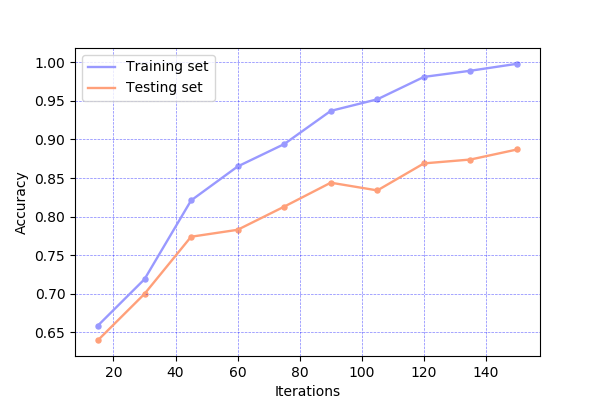
\includegraphics[width=0.45\linewidth]{img/svm_baseline_splice.png}
	}
	\subfigure[Satimage]{
		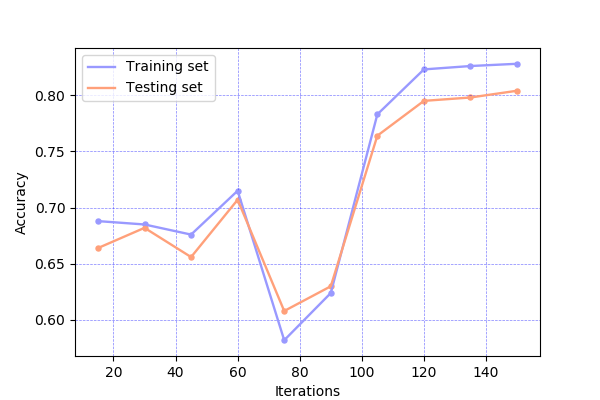
\includegraphics[width=0.45\linewidth]{img/svm_baseline_sat.png}
	}
	\caption{The baseline of SVM.}
	\label{fig:svm-baseline}
\end{figure}

\subsubsection{Kernel}

The ability of SVM might be constrainted when dealing with non-linear features, where kernel trick could resolve this issue. Nevertheless, a successful choice of kernel is still based on experience or luck. I apply several kernels to SVM and get the following results (Fig. \ref{fig:svm-kernel}).

\begin{figure}[H]
	\centering
	\subfigure[Splice-Training Set]{
		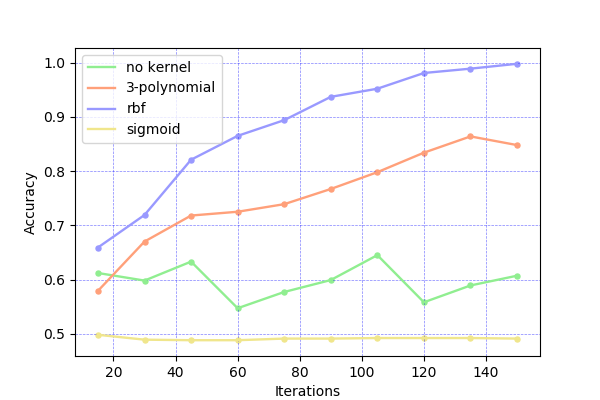
\includegraphics[width=0.45\linewidth]{img/svm_kernel_splice_tr.png}
	}
	\subfigure[Splice-Tetsing Set]{
		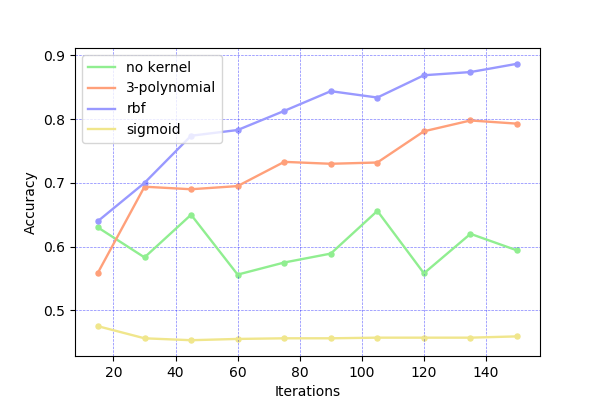
\includegraphics[width=0.45\linewidth]{img/svm_kernel_splice_t.png}
	}
	\subfigure[Satimage-Training Set]{
		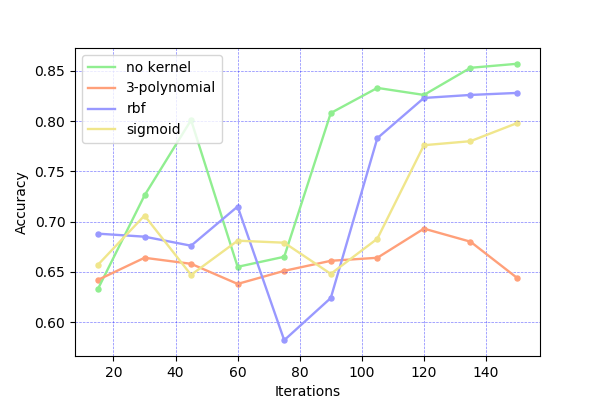
\includegraphics[width=0.45\linewidth]{img/svm_kernel_sat_tr.png}
	}
	\subfigure[Satimage-Testing Set]{
		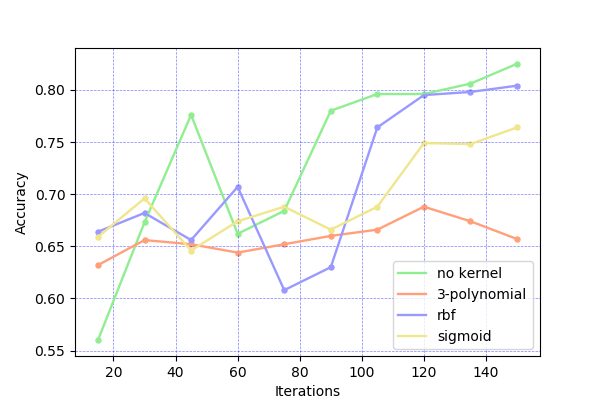
\includegraphics[width=0.45\linewidth]{img/svm_kernel_sat_t.png}
	}
	\caption{The performances of SVM under different kernels.}
	\label{fig:svm-kernel}
\end{figure}

It is apparent that the effect of these kernels differ greatly. Rbf (Radial Basis Function) kernel is best for \textit{splice} while no kernel function is the best choice for \textit{satimage}. 

\vspace{0.01\linewidth}
Additionally, the selection of specific parameters of a kernel would also affect the results. I test polynomial kernel with different numbers of power, the test error can refer to Tab. \ref{tab:kernel-poly}.

\begin{table}[H]
	\renewcommand\arraystretch{1.35}
	\caption{The performances of polynomial kernel under different powers}
	\label{tab:kernel-poly}
	\centering
	
	\begin{tabular}{c|c|c}
		\centering
		Number of Power & Testing Error(Splice) & Testing Error(Satimage) \\
		\hline
		
		2 & 0.786 & 0.635 \\
		3 & 0.857 & 0.666 \\
		4 & 0.865 & 0.505 \\
		5 & 0.871 & 0.554 \\
		6 & 0.880 & 0.488 \\
		7 & 0.874 & 0.512 \\
		8 & 0.864 & 0.477 \\
		9 & 0.867 & 0.528 \\
		10 & 0.851 & 0.403 \\
	\end{tabular}
\end{table}

The trend reflected in the table is that higher power can reduce training error, but lead to more test error in the meantime. Still, the performance would also drop a lot in both training set and testing set when the power is too large. This result also proves the significance fo choosing the complexity of model properly.

\subsubsection{Penalty Parameter}

Although SVM would encounter difficulties on non-linear data, it can still handle slightly non-separable data via soft-margin technique (transforming the optimization object into $\dfrac{1}{2}w^Tw+C\sum\limits_{n=1}^{N}\xi_n$), where the penalty parameter $C$ is critical for classification performance. I have tried the $C$ of different orders of magnitudes, and the results can be found in Fig. \ref{fig:svm-penalty}.

\begin{figure}[H]
	\centering
	\subfigure[Splice]{
		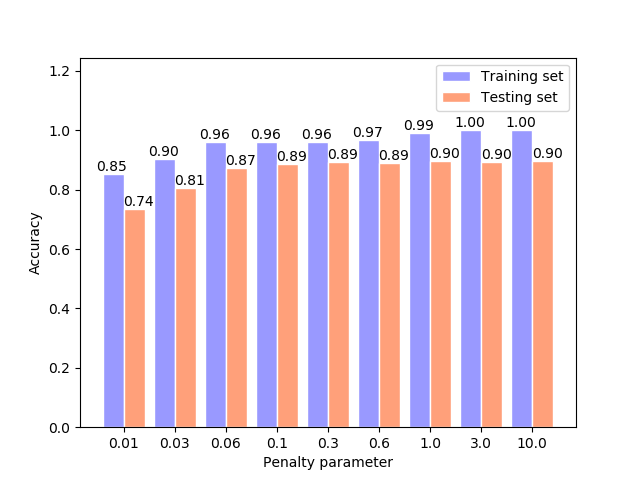
\includegraphics[width=0.45\linewidth]{img/svm_penalty_splice.png}
	}
	\subfigure[Satimage]{
		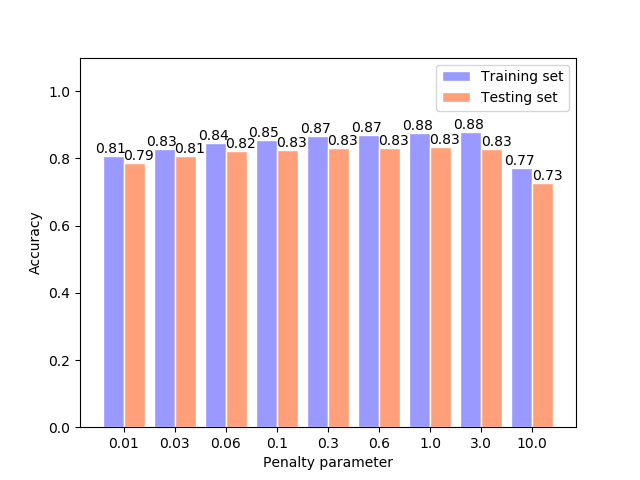
\includegraphics[width=0.45\linewidth]{img/svm_penalty_sat.png}
	}
	\caption{The performances of SVM under different penalty parameter $C$.}
	\label{fig:svm-penalty}
\end{figure}

According to the results, the introduction of $C$ is sometimes beneficial to the classification. More specifically, proper $C$ could improve the performance of SVM while excessive $C$ might produce additional errors. In general, the circumstances might vary a little bit according to the data, where $C$ should be determined by large scale of experiments.

\subsubsection{Dimension of Features}



\begin{figure}[H]
	\centering
	\subfigure[Splice-Training Set]{
		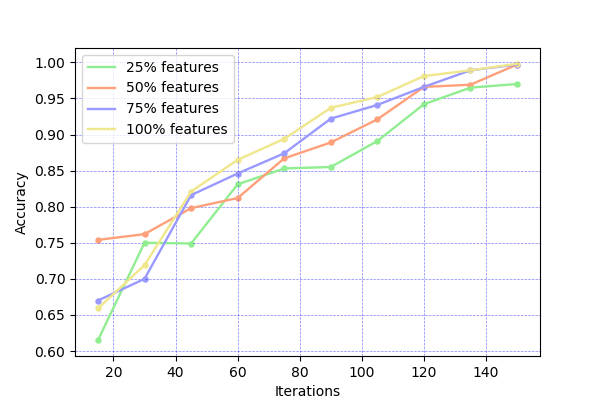
\includegraphics[width=0.45\linewidth]{img/svm_dim_splice_tr.png}
	}
	\subfigure[Splice-Tetsing Set]{
		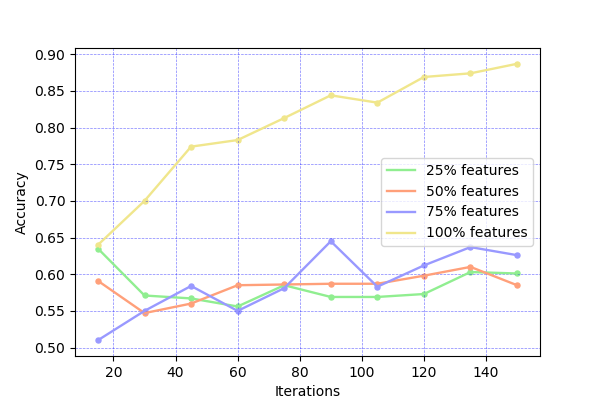
\includegraphics[width=0.45\linewidth]{img/svm_dim_splice_t.png}
	}
	\subfigure[Satimage-Training Set]{
		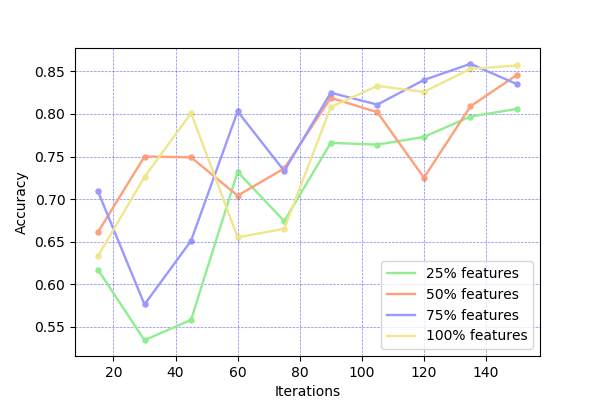
\includegraphics[width=0.45\linewidth]{img/svm_dim_sat_tr.png}
	}
	\subfigure[Satimage-Testing Set]{
		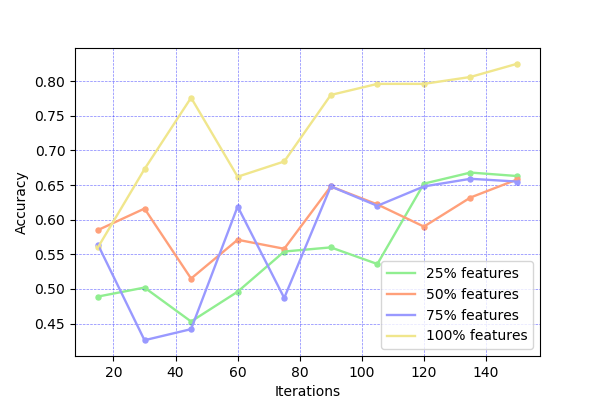
\includegraphics[width=0.45\linewidth]{img/svm_dim_sat_t.png}
	}
	\caption{The performances of SVM under different dimensions of features.}
	\label{fig:svm-dim}
\end{figure}

\subsection{Neural Network}

In this section, I would also show the performances of MLP in the two datasets under different configurations (e.g. optimization algorithms, network architectures). In the meantime, I would also analyze each result concisely.

\vspace{0.01\linewidth}
Same as Sec. \ref{sec:svm}, I conduct the following experiments based on default parameters in \textit{sklearn}. Some important parameters are shown in Tab. \ref{tab:default-para-mlp} and the baseline model can refer to Fig. \ref{fig:mlp-baseline}.

\begin{table}[H]
	\renewcommand\arraystretch{1.35}
	\caption{Some important default parameters of MLP experiments}
	\label{tab:default-para-mlp}
	\centering
	
	\begin{tabular}{c|c|c}
		\centering
		Name & Meaning & Value \\
		\hline
		\hline
		
		hidden\_layer\_sizes & the size of hidden layers & (100,) \\
		activation & activation function for the hidden layer & relu \\
		solver & the solver for weight optimization & adam \\
		alpha & L2 penalty (regularization term) parameter & 0.0001 \\
		batch\_size & size of minibatches for stochastic optimizers & min(200, n\_samples) \\
		learning\_rate\_init & the initial learning rate used & 0.001 \\
		power\_t & the exponent for inverse scaling learning rate & 0.5 \\
		tol & tolerance for the optimization & 1e-4 \\
		
	\end{tabular}
\end{table}

\begin{figure}[H]
	\centering
	\subfigure[Splice]{
		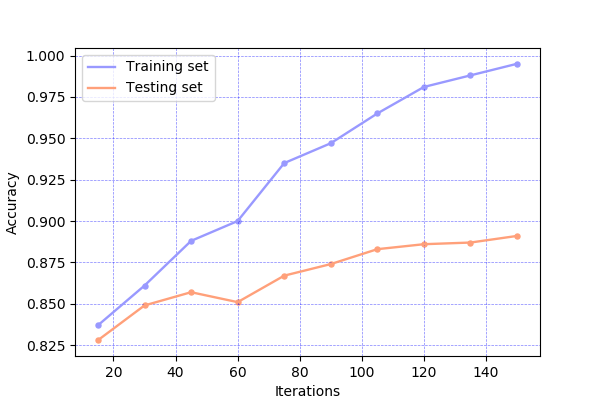
\includegraphics[width=0.45\linewidth]{img/mlp_baseline_splice.png}
	}
	\subfigure[Satimage]{
		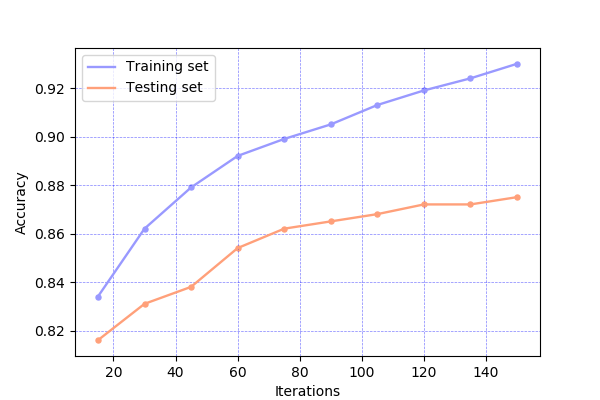
\includegraphics[width=0.45\linewidth]{img/mlp_baseline_sat.png}
	}
	\caption{The baseline of MLP.}
	\label{fig:mlp-baseline}
\end{figure}

\subsubsection{Optimization Algorithm}

\begin{figure}[H]
	\centering
	\subfigure[Splice-Training Set]{
		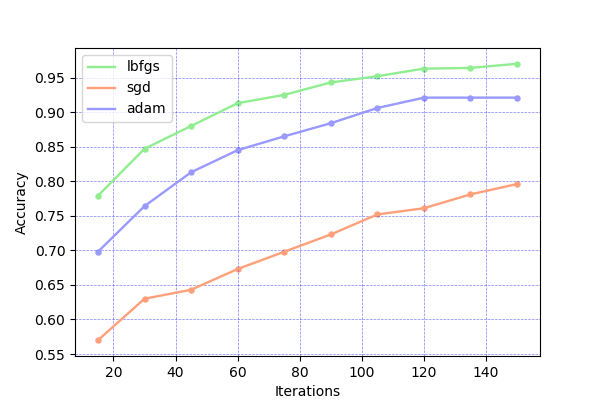
\includegraphics[width=0.45\linewidth]{img/mlp_optimizer_splice_tr.png}
	}
	\subfigure[Splice-Tetsing Set]{
		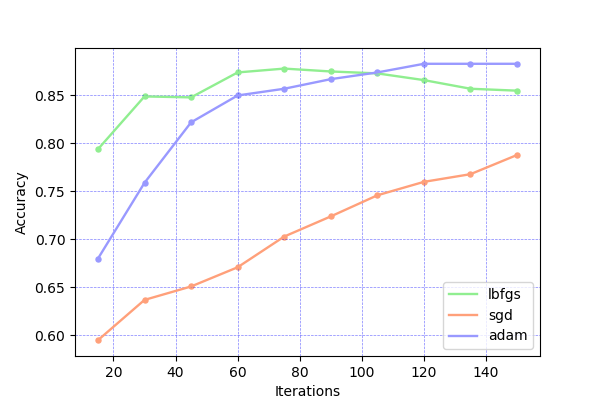
\includegraphics[width=0.45\linewidth]{img/mlp_optimizer_splice_t.png}
	}
	\subfigure[Satimage-Training Set]{
		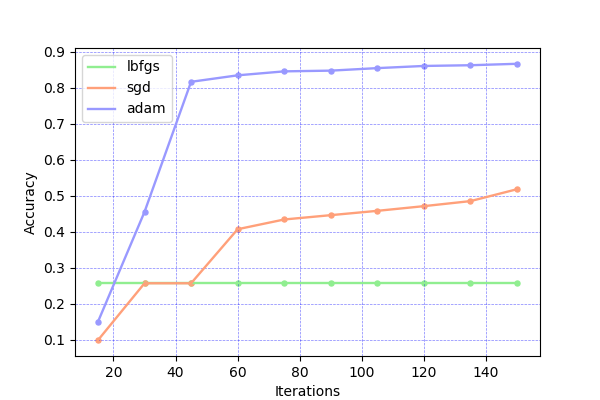
\includegraphics[width=0.45\linewidth]{img/mlp_optimizer_sat_tr.png}
	}
	\subfigure[Satimage-Testing Set]{
		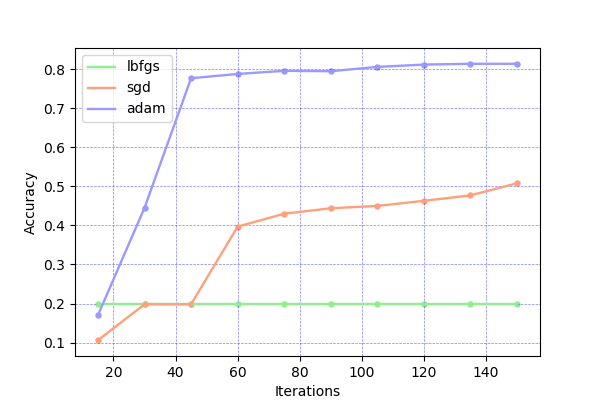
\includegraphics[width=0.45\linewidth]{img/mlp_optimizer_sat_t.png}
	}
	\caption{The performances of MLP under different optimization algorithms.}
	\label{fig:mlp-optimizer}
\end{figure}

\subsubsection{Activation Function}

\begin{figure}[H]
	\centering
	\subfigure[Splice-Training Set]{
		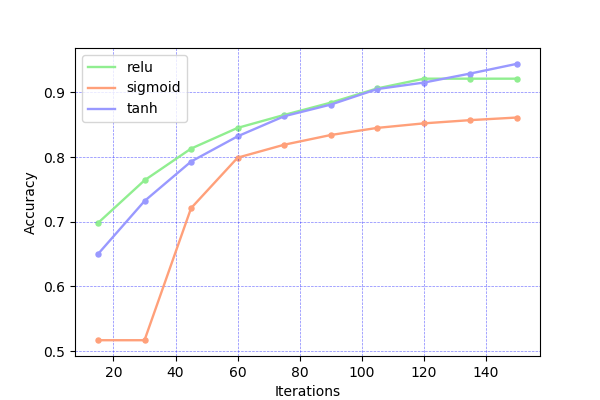
\includegraphics[width=0.45\linewidth]{img/mlp_activation_splice_tr.png}
	}
	\subfigure[Splice-Tetsing Set]{
		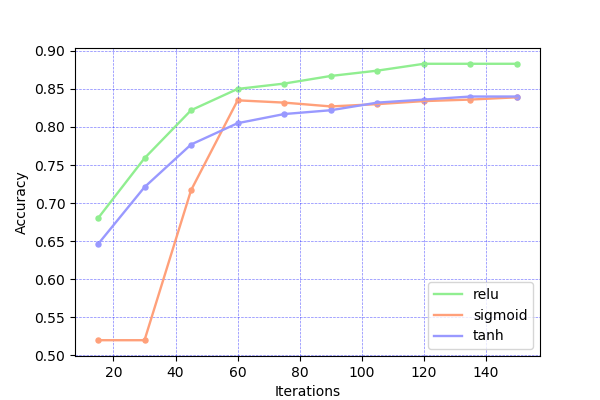
\includegraphics[width=0.45\linewidth]{img/mlp_activation_splice_t.png}
	}
	\subfigure[Satimage-Training Set]{
		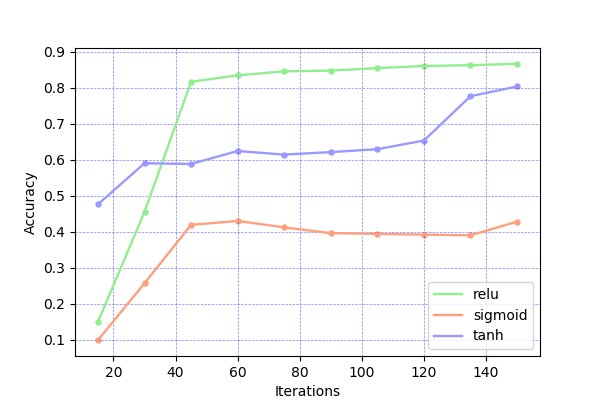
\includegraphics[width=0.45\linewidth]{img/mlp_activation_sat_tr.png}
	}
	\subfigure[Satimage-Testing Set]{
		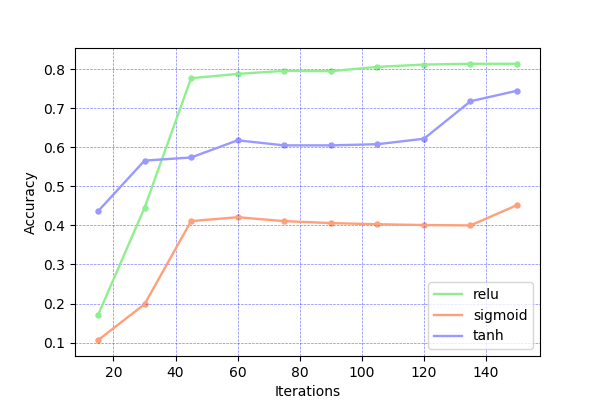
\includegraphics[width=0.45\linewidth]{img/mlp_activation_sat_t.png}
	}
	\caption{The performances of MLP under different activation functions.}
	\label{fig:mlp-activation}
\end{figure}

\subsubsection{Learning Rate}

\begin{figure}[H]
	\centering
	\subfigure[Splice]{
		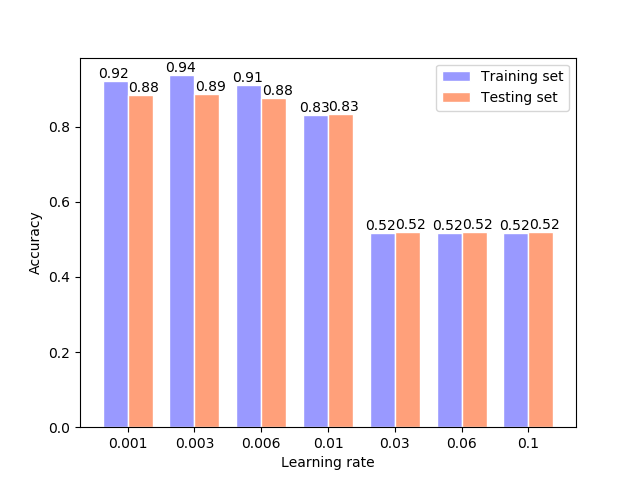
\includegraphics[width=0.45\linewidth]{img/mlp_lr_splice.png}
	}
	\subfigure[Satimage]{
		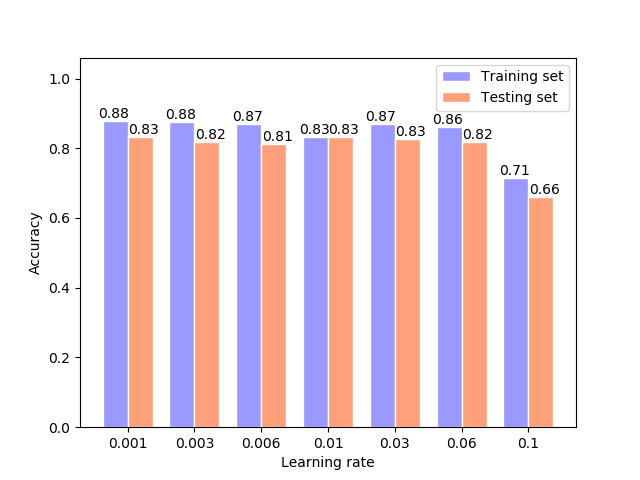
\includegraphics[width=0.45\linewidth]{img/mlp_lr_sat.png}
	}
	\caption{The performances of MLP under different learning rate.}
	\label{fig:mlp-lr}
\end{figure}

\subsubsection{Network Architecture}

\begin{figure}[H]
	\centering
	\subfigure[Splice-Training Set]{
		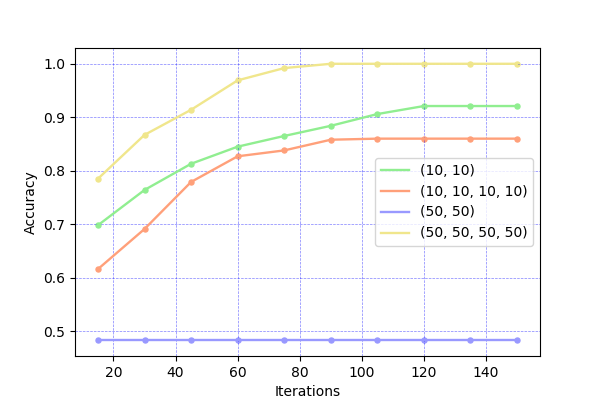
\includegraphics[width=0.45\linewidth]{img/mlp_archi_splice_tr.png}
	}
	\subfigure[Splice-Tetsing Set]{
		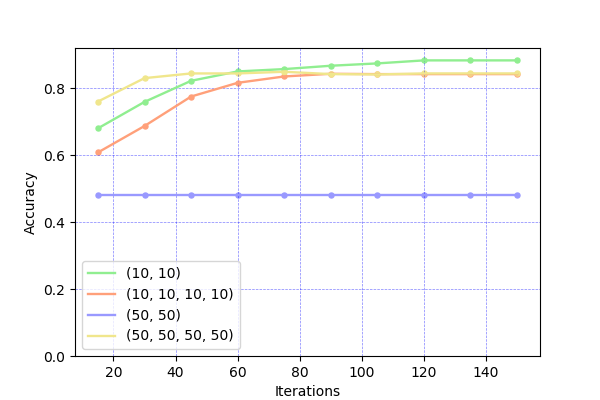
\includegraphics[width=0.45\linewidth]{img/mlp_archi_splice_t.png}
	}
	\subfigure[Satimage-Training Set]{
		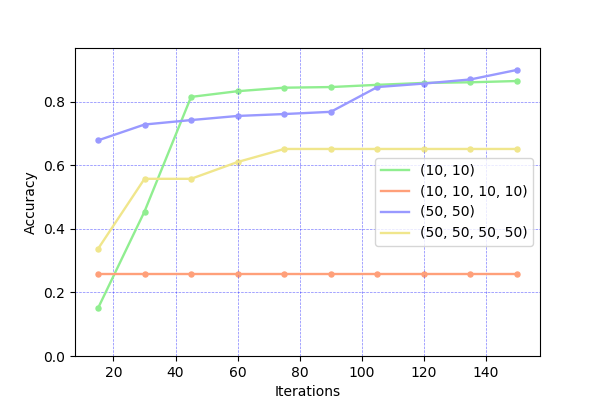
\includegraphics[width=0.45\linewidth]{img/mlp_archi_sat_tr.png}
	}
	\subfigure[Satimage-Testing Set]{
		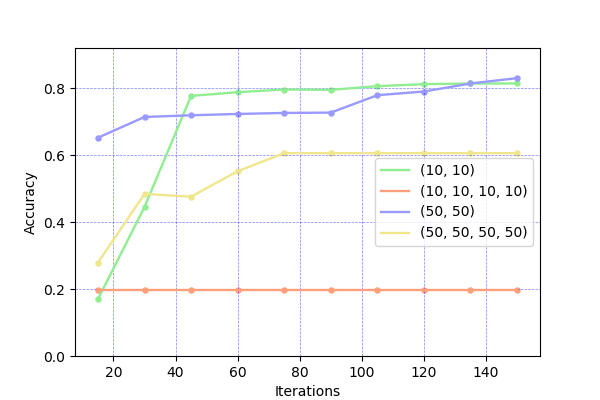
\includegraphics[width=0.45\linewidth]{img/mlp_archi_sat_t.png}
	}
	\caption{The performances of MLP under different network architectures.}
	\label{fig:mlp-archi}
\end{figure}

\subsubsection{Dimension of Features}

\begin{figure}[H]
	\centering
	\subfigure[Splice-Training Set]{
		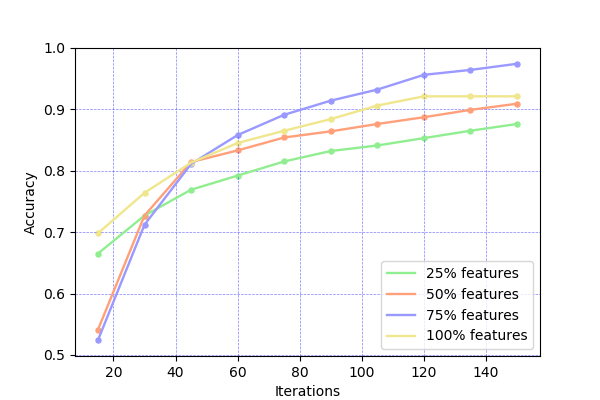
\includegraphics[width=0.45\linewidth]{img/mlp_dim_splice_tr.png}
	}
	\subfigure[Splice-Tetsing Set]{
		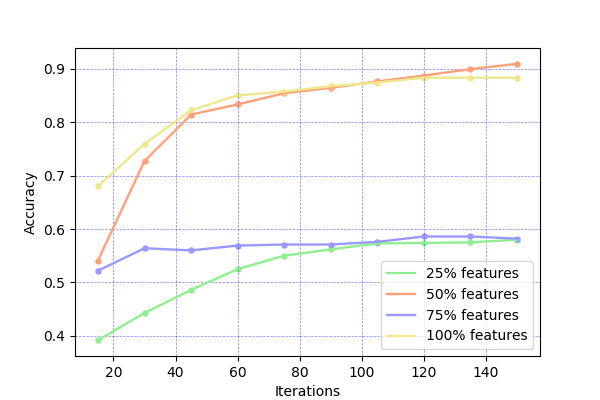
\includegraphics[width=0.45\linewidth]{img/mlp_dim_splice_t.png}
	}
	\subfigure[Satimage-Training Set]{
		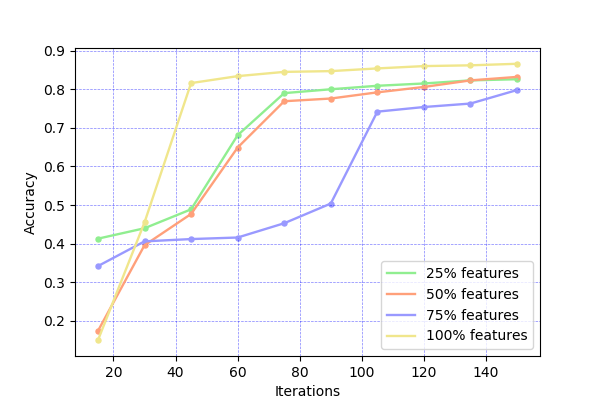
\includegraphics[width=0.45\linewidth]{img/mlp_dim_sat_tr.png}
	}
	\subfigure[Satimage-Testing Set]{
		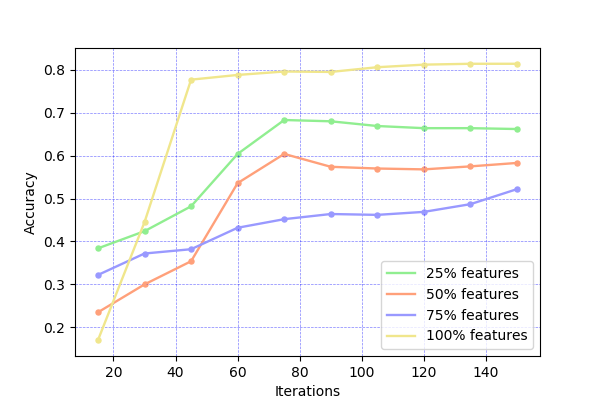
\includegraphics[width=0.45\linewidth]{img/mlp_dim_sat_t.png}
	}
	\caption{The performances of MLP under different dimensions of features.}
	\label{fig:mlp-dim}
\end{figure}

\section{Comparison Between SVM and Deep Learning Algorithm Benchmark}

\newpage
\begin{appendix}
\section{Appendix}

\subsection{Details of Datasets in Experiments}
\label{apd:dataset}

\subsubsection{Splice \cite{splice}}

Basically, according to the biological knowledge, splice junctions are points on a DNA sequence at which `superfluous' DNA is removed during the process of protein creation in higher organisms.

\vspace{0.01\linewidth}
Splice dataset aims to recognize two classes of splice junctions, given a DNA sequence, the boundaries between exons (the parts of the DNA sequence retained after splicing) and introns (the parts of the DNA sequence that are spliced out).

\subsubsection{Satimage \cite{satimage}}

Satimage dataset is also called \textbf{satalog} dataset. It contains multi-spectral values of pixels in 3 $\times$ 3 neighbourhoods in satellite images, and the classification associated with the central pixel in each neighbourhood.

\vspace{0.01\linewidth}
As a classification dataset, the aim of satimage is to predict the classification, given the multi-spectral values. In the sample database, the class of a pixel is coded as a number.

\subsubsection{ConvexNonConvex \cite{convex}}

The ConvexNonConvex dataset consists of convex regions with pixels of value 255. Such regions are constructed via the intersection of a number of half-planes whose location and orientation were chosen uniformly at random. In the meanwhile, the number of half-planes is also sampled randomly according to a geometric distribution with parameter 0.195.

\vspace{0.01\linewidth}
To ensure the validity of the data, a candidate convex image is rejected once there are less than 19 pixels in it.


\end{appendix}

\bibliographystyle{ieeetr}
\bibliography{bio}

\end{document}